\documentclass{article}\usepackage[]{graphicx}\usepackage[]{color}
%% maxwidth is the original width if it is less than linewidth
%% otherwise use linewidth (to make sure the graphics do not exceed the margin)
\makeatletter
\def\maxwidth{ %
  \ifdim\Gin@nat@width>\linewidth
    \linewidth
  \else
    \Gin@nat@width
  \fi
}
\makeatother

\definecolor{fgcolor}{rgb}{0.345, 0.345, 0.345}
\newcommand{\hlnum}[1]{\textcolor[rgb]{0.686,0.059,0.569}{#1}}%
\newcommand{\hlstr}[1]{\textcolor[rgb]{0.192,0.494,0.8}{#1}}%
\newcommand{\hlcom}[1]{\textcolor[rgb]{0.678,0.584,0.686}{\textit{#1}}}%
\newcommand{\hlopt}[1]{\textcolor[rgb]{0,0,0}{#1}}%
\newcommand{\hlstd}[1]{\textcolor[rgb]{0.345,0.345,0.345}{#1}}%
\newcommand{\hlkwa}[1]{\textcolor[rgb]{0.161,0.373,0.58}{\textbf{#1}}}%
\newcommand{\hlkwb}[1]{\textcolor[rgb]{0.69,0.353,0.396}{#1}}%
\newcommand{\hlkwc}[1]{\textcolor[rgb]{0.333,0.667,0.333}{#1}}%
\newcommand{\hlkwd}[1]{\textcolor[rgb]{0.737,0.353,0.396}{\textbf{#1}}}%

\usepackage{framed}
\makeatletter
\newenvironment{kframe}{%
 \def\at@end@of@kframe{}%
 \ifinner\ifhmode%
  \def\at@end@of@kframe{\end{minipage}}%
  \begin{minipage}{\columnwidth}%
 \fi\fi%
 \def\FrameCommand##1{\hskip\@totalleftmargin \hskip-\fboxsep
 \colorbox{shadecolor}{##1}\hskip-\fboxsep
     % There is no \\@totalrightmargin, so:
     \hskip-\linewidth \hskip-\@totalleftmargin \hskip\columnwidth}%
 \MakeFramed {\advance\hsize-\width
   \@totalleftmargin\z@ \linewidth\hsize
   \@setminipage}}%
 {\par\unskip\endMakeFramed%
 \at@end@of@kframe}
\makeatother

\definecolor{shadecolor}{rgb}{.97, .97, .97}
\definecolor{messagecolor}{rgb}{0, 0, 0}
\definecolor{warningcolor}{rgb}{1, 0, 1}
\definecolor{errorcolor}{rgb}{1, 0, 0}
\newenvironment{knitrout}{}{} % an empty environment to be redefined in TeX

\usepackage{alltt}
\usepackage[sc]{mathpazo}
\usepackage[T1]{fontenc}
\usepackage{geometry}
\geometry{verbose,tmargin=2.5cm,bmargin=2.5cm,lmargin=2.5cm,rmargin=2.5cm}
\setcounter{secnumdepth}{2}
\setcounter{tocdepth}{2}
\usepackage{url}
\usepackage[unicode=true,pdfusetitle,
 bookmarks=true,bookmarksnumbered=true,bookmarksopen=true,bookmarksopenlevel=2,
 breaklinks=false,pdfborder={0 0 1},backref=false,colorlinks=false]
 {hyperref}
\hypersetup{
 pdfstartview={XYZ null null 1}}
\usepackage{breakurl}
\IfFileExists{upquote.sty}{\usepackage{upquote}}{}
\begin{document}


\section*{Problem 3}

\begin{knitrout}
\definecolor{shadecolor}{rgb}{0.969, 0.969, 0.969}\color{fgcolor}\begin{kframe}
\begin{alltt}
\hlcom{# We constructed a function called rgene to generate the of a circle with}
\hlcom{# radius r}
\hlkwd{set.seed}\hlstd{(}\hlnum{0}\hlstd{)}
\hlstd{rgene} \hlkwb{<-} \hlkwa{function}\hlstd{(}\hlkwc{r}\hlstd{) \{}
    \hlstd{theta} \hlkwb{<-} \hlkwd{runif}\hlstd{(}\hlnum{150}\hlstd{,} \hlkwc{min} \hlstd{=} \hlopt{-}\hlstd{pi,} \hlkwc{max} \hlstd{= pi)}
    \hlstd{x} \hlkwb{<-} \hlstd{r} \hlopt{*} \hlkwd{cos}\hlstd{(theta)} \hlopt{+} \hlkwd{rnorm}\hlstd{(}\hlnum{150}\hlstd{,} \hlkwc{mean} \hlstd{=} \hlnum{0}\hlstd{,} \hlkwc{sd} \hlstd{=} \hlnum{0.25}\hlstd{)}
    \hlstd{y} \hlkwb{<-} \hlstd{r} \hlopt{*} \hlkwd{sin}\hlstd{(theta)} \hlopt{+} \hlkwd{rnorm}\hlstd{(}\hlnum{150}\hlstd{,} \hlkwc{mean} \hlstd{=} \hlnum{0}\hlstd{,} \hlkwc{sd} \hlstd{=} \hlnum{0.25}\hlstd{)}
    \hlkwd{return}\hlstd{(}\hlkwd{cbind}\hlstd{(}\hlkwc{x} \hlstd{= x,} \hlkwc{y} \hlstd{= y))}
\hlstd{\}}
\hlstd{X} \hlkwb{<-} \hlkwd{rgene}\hlstd{(}\hlnum{5}\hlstd{)}
\hlstd{Y} \hlkwb{<-} \hlkwd{rgene}\hlstd{(}\hlnum{2.8}\hlstd{)}
\hlstd{Z} \hlkwb{<-} \hlkwd{rgene}\hlstd{(}\hlnum{1}\hlstd{)}
\hlcom{# Draw the plot of graph}
\hlkwd{plot}\hlstd{(X,} \hlkwc{main} \hlstd{=} \hlstr{"Simulated Data Points"}\hlstd{)}
\hlkwd{points}\hlstd{(Y,} \hlkwc{col} \hlstd{=} \hlstr{"red"}\hlstd{)}
\hlkwd{points}\hlstd{(Z,} \hlkwc{col} \hlstd{=} \hlstr{"blue"}\hlstd{)}
\end{alltt}
\end{kframe}

{\centering 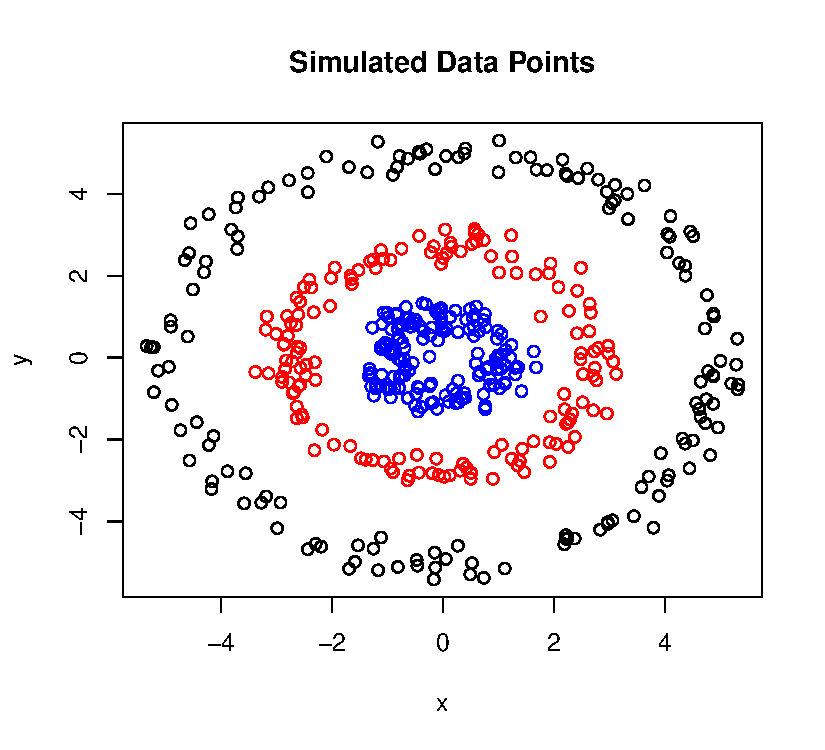
\includegraphics[width=\maxwidth]{figure/minimal-Problem_31} 

}


\begin{kframe}\begin{alltt}
\hlcom{# Spectral Clustering}
\hlkwd{library}\hlstd{(kernlab)}
\hlstd{s_data} \hlkwb{<-} \hlkwd{rbind}\hlstd{(X, Y, Z)}
\hlstd{spec_cl} \hlkwb{<-} \hlkwd{specc}\hlstd{(s_data,} \hlkwc{centers} \hlstd{=} \hlnum{3}\hlstd{)}
\hlcom{# It is a really accurate clustering}
\hlkwd{plot}\hlstd{(s_data,} \hlkwc{pch} \hlstd{= spec_cl,} \hlkwc{main} \hlstd{=} \hlstr{"Spectral Clustered Points Denoted Using Different Symbols"}\hlstd{)}
\end{alltt}
\end{kframe}

{\centering 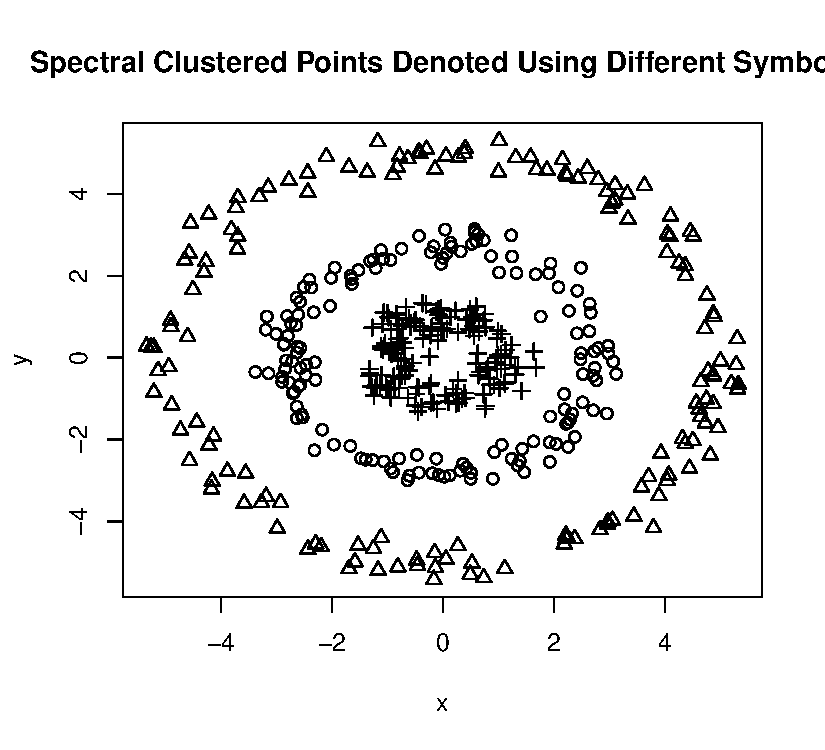
\includegraphics[width=\maxwidth]{figure/minimal-Problem_32} 

}


\begin{kframe}\begin{alltt}
\hlcom{# Kernel PCA}
\hlstd{s_kpc} \hlkwb{<-} \hlkwd{kpca}\hlstd{(s_data,} \hlkwc{kernel} \hlstd{=} \hlstr{"rbfdot"}\hlstd{,} \hlkwd{list}\hlstd{(}\hlkwc{sigma} \hlstd{=} \hlnum{0.7}\hlstd{))}
\hlkwd{plot}\hlstd{(}\hlkwd{rotated}\hlstd{(s_kpc)[,} \hlnum{1}\hlstd{],} \hlkwd{rotated}\hlstd{(s_kpc)[,} \hlnum{2}\hlstd{],} \hlkwc{main} \hlstd{=} \hlstr{"Rotated Data using Kernel PCA"}\hlstd{)}
\end{alltt}
\end{kframe}

{\centering 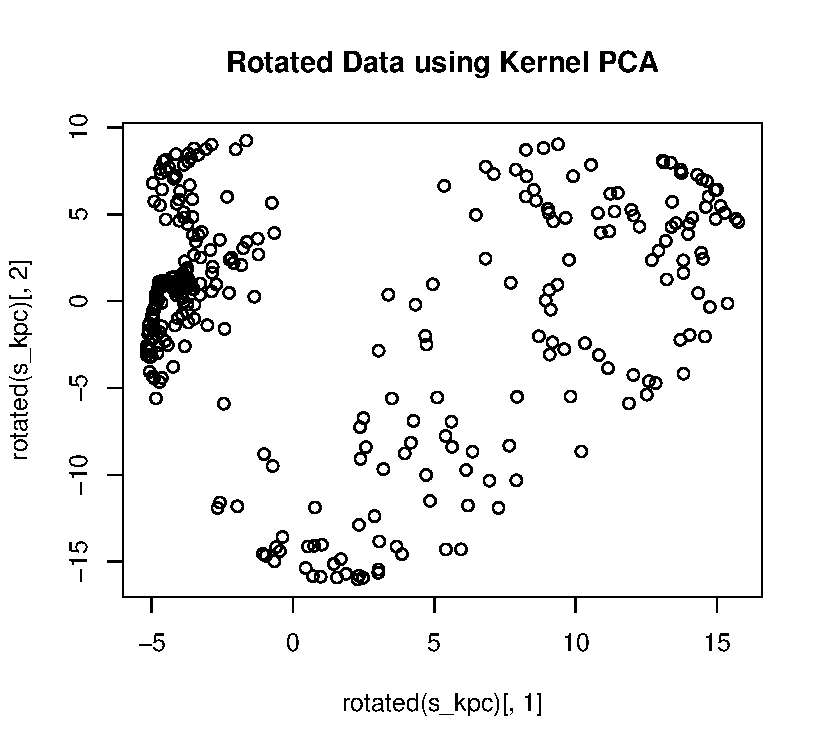
\includegraphics[width=\maxwidth]{figure/minimal-Problem_33} 

}


\begin{kframe}\begin{alltt}
\hlcom{# Comment: Using kernel PCA, we can see that there are three parts of}
\hlcom{# points that can be grouped.}
\hlcom{# PCA}
\hlstd{s_pc} \hlkwb{<-} \hlkwd{prcomp}\hlstd{(s_data,} \hlkwc{rtex} \hlstd{=} \hlnum{TRUE}\hlstd{,} \hlkwc{scale} \hlstd{=} \hlnum{TRUE}\hlstd{)}
\hlkwd{plot}\hlstd{(s_pc}\hlopt{$}\hlstd{x,} \hlkwc{main} \hlstd{=} \hlstr{"Rotated Data Using PCA"}\hlstd{)}
\end{alltt}
\end{kframe}

{\centering 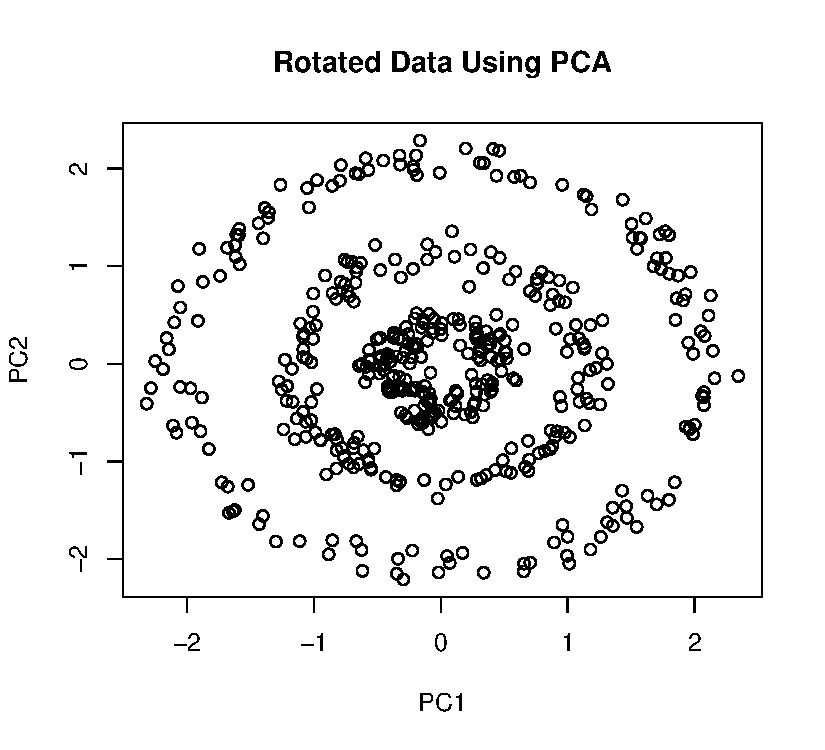
\includegraphics[width=\maxwidth]{figure/minimal-Problem_34} 

}


\begin{kframe}\begin{alltt}
# Comment: Obviously, PCA cannot help us to cluster the data, which is
# reasonable since what we have done is only rotating the coordinates;
# however, it does not change anything since the data spread like
# circles.
\end{alltt}
\end{kframe}
\end{knitrout}

\end{document}


